\subsection{Drift System Implementation}
\label{driftimplementation}

The last chapter conceptionally introduced the \textit{Drift language}
as well as the \textit{Drift Shell}. This chapter will introduce
the current implementation of the \textit{Drift} back-end system,
based on the ideas presented so far.

Both, the Drift language and shell, are heavily influenced
by the idea that most of the semantics of programming for us
programmers is contained within the \textit{names} that are being
used. Which makes it hard to differentiate between which
functionality is defined by the language and which by the shell.

One example of this would be the variable-space which is
defined to consist of names and namespaces only, forming the same
kind of namespace-tree as a traditional UNIX file system.
This tree and variable-space can be walked using the language
keywords \texttt{ls} and \texttt{cd} which are therefor implemented
as shell built-ins.

Furthermore some assumptions and invariants of the underlying
system's behavior have also been sketched, based on the ideas
introduced by chapters \ref{LanguageOfTheSystem} - \ref{bretvictor}.
One example of this would be, that names can be removed from
the pseudo-global namespace emulated by each shell session,
but the data that is referenced by this name needs to be
held on to and made available by the system in case any
running service is still consuming from this data.
So using the concepts of Rich Hickey as introduced in
chapter \ref{LanguageOfTheSystem}, from the user perspective
names behave like places but from the system perspective
data behaves like values.

Another aspect that has already been scratched upon, is the
idea that data should be made observable as soon as it is
available. This is based on the realization that batch
processing is only a special case of stream processing.
In other words: batch data is just streaming data with all
the stream snippets that would otherwise trickle down
over time having already arrived. Therefor any system that
is able to deal with the fact that data might only arrive
as delayed chunks, will naturally be able to deal with a
delay size of 0.

So in order to build a back-end system that supports these
assumptions, one needs to first define the basic tasks of
the front-end (the shell), the back-end and how they interface
with one another. Fig.\ref{system-abstract} shows the
basic idea of how this looks in the current implementation.

\begin{figure}[h]
  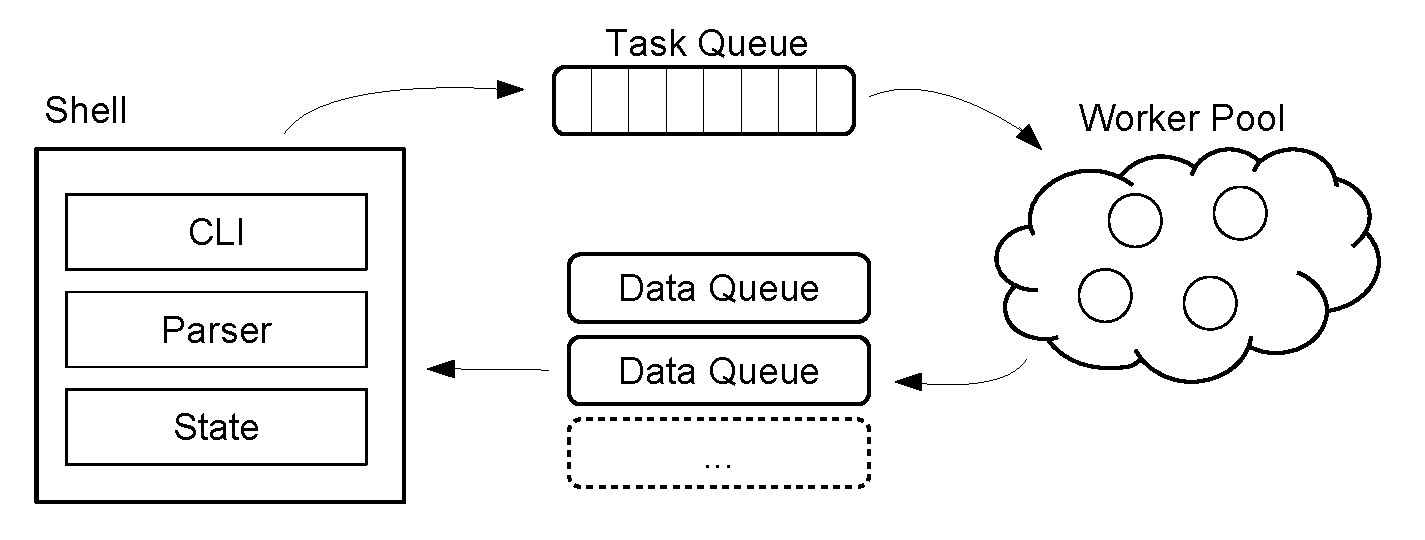
\includegraphics[scale=0.6, keepaspectratio]{system_abstract.pdf}
  \caption{Abstract architecture of the Drift front-end and back-end
           and the interfacing between the two.}
  \label{system-abstract}
\end{figure}

The shell's job is to present the user with a textual interface
and send any valid commands as tasks to the system. Therefor
the shell is \textit{not} part of the system per se. It runs
on the user's machine and connects to the system via network.
This means the user can interface with the system virtually from
anywhere.
This might seem insignificant but another vital task of
the shell is to present the user with its own
seperated and stateful environment. Each session defines its own
names and never interferes with any other ongoing session, in the
same way that a user working on a UNIX system is isolated from
and should never even notice any other user.

So in order to provide these guarantess, the shell mainly consists of
three parts. All parts and therefor the shell itself are currently
implemented in Java 8 (official version 1.8).
The \textit{command line interface} (CLI) deals with presenting
the shell to the user and handling any input and output from
and to the user. Any input received is passed to the
language parser which was generated using the ANTLR parser
generator (version 4) \cite{antlr}. Additionally in the
parsing layer the shell connects to the service registry which
is not yet shown in the high-level overview of Fig.\ref{system-abstract}.
If any syntactical errors are found or the services do not fit
the specification stored in the service registry, a specific error
message is printed to the screen.

It is important to note however, that in the current implementation
every command entered by the user is fact-checked with the help
of the service registry. This could be optimized by caching any
information retreived about a service in the client shell, therefor
saving round-trips over the network. However, such a caching
infrastructure would, depending on the change rate of the entries
in the service registry, be vulnerable to stale entries. Therefor
some form of cache invalidation or cache coherency protocol would
be needed, updating \textit{all} the client caches
whenever an entry in the service registry changes.
This was considered future work, as will be discussed in the
appropriate chapter, chapter \ref{futurework}.

The third aspect of the shell is the internal state of the session
which consists of two things. A name table that maps the names the
user created in her session to the names that are used withinin the
system and the history log for each name and namesapce in the session.

The history log for each name (or namespace) is itself implemented as a
\textit{persistent data structure} \cite{pds-paper}, \cite{pds-book}:
an immutable append-only log, just like Datomic as presented in
chapter \ref{datomic}. Therefor each name that is
created, either via an import or a service invocation, gets its
own history log. Each name that occured in the command
that created the name is stored as a reference into the
history log of that name and therefor the value of that name
at the point in time when the command was issued.

Over time this creates a reference tree in which the entry of a name
points to old values of the names that were used to create it. This
tree can then of course be traversed using the history query
operators \texttt{?} and \texttt{??} as introduced in the last
chapter, chapter \ref{driftlang}. This is also one aspect of the
implementation of the closure behavior of service invocations as
demanded by the Drift language, as was also presented in the last
chapter.
\newline

When the command that was entered by the user is valid, a
task description is generated and send to the \textit{task queue}.
There is only  \textit{one} designated task queue. The task description
itself is also generated by the parsing layer of the shell.

Since the Drift language does not feature very much syntactical
concepts it has a reasonably straight forward grammar. So it could
be argued that the usage of the ANTLR parser generator might be
overengineering, since most of the more advanced tooling offered
by the ANTLR tool is never used. However, given the structure
of the parser generated by the ANTLR parser generator, parsing
a command given by the user naturally builds up a command
description structure, by visiting all the elements of the
command down to every name. Therefor the use of ANTLR was not only for
automatically generating the parser itself but also for generating the
task description as a byproduct of parsing each command.

This task description fulfills two purposes. For one it serves
as the obvious task description and contains every information
needed by a worker to execute the given task. But it also serves
as an identifier because in order to deliver the guarantees
demanded by the semantics of the  Driftlanguage, one invariant of
the system is that the execution of services is \textit{deterministic}.

This means that given two service invocations with the exact same
input data, the results of both invocations must be identical.
From this it follows that since the result of a task only depends
on its direct inputs and not on any further state of the system,
the task invocation description, the command that created the
task, can be used as an identifier for the result of the task.

This is done via hashing the task description structure that was
generated by parsing the given command. The resulting hash value
is used to uniquely and globally identify the result of the command
in all of the system. It is this hash that is stored in the name
table of the shell, that maps the names given by the user to
their hashes, their global system names.
\newline

Nonetheless, in order for the workers to be able to execute a
task, the whole task description structure is send to the task
queue. On the other end of the task queue there is a pool of
workers. In order to allow for these workers to achieve hight
scalability and fault tolerance, it is adviced to run each worker
on a seperate machine, as was done in the current implementation.

Any free worker will then pull the new task out of the task queue,
execute the task according to the task description and produce its
result into another message queue, a \textit{data queue}.

The name of the resulting data queue is of course the hash of the
task description structure the worker received. Therefor both,
the shell and the system exchange the full task descriptions
but use the hash of the description in order to identify where
to consume from or produce to. So when the user queries the name,
that was bound to the result of the command that was entered
earlier, the shell looks up the hash-name from the user-defined
name and consumes from the data queue with that name in order to show
the result to the user.
\newline

The whole data layer of the system is implemented using distributed
message queues. This was done because of the demand of the Drift
language that data needs to observable as soon as it is available.
Earlier versions featured a distributed file system like the
\textit{Hadoop Distributed File System} (HDFS). Unfortunately it
is absolutely not trivial to implement \textit{any} form of
data streaming capabilities on top of HDFS, since the file
abstraction provided by HDFS does not allow for any contention
or publish-subscribe functionality.

At the time of this writing most of the available distributed
file systems are still struggling with even providing basic
POSIX conformability. HDFS for example is \textit{not} POSIX
conform. Unfortunately, even if it was, this wouldn't actually be of
much help, because the POSIX file system API does not provide
any mechanisms for being notified for file change. Eventhough
the Linux kernel does implement such an API, namely the
\textit{inotify} interface, this is mostly ignored by both,
the POSIX standard and the distributed file system community.

Luckily the distributed message queue community can be considered
very active in this regard which is why not only coordination
and communication is done via message queues but also storage
and persistence. This means that the shell can listen on the
resulting data queue represented by name and as soon as the first
data token is produced by a worker into that queue, consume this
token and present it to the user.
\newline

In order to illustrate the detailed processing of a task,
Fig.\ref{system2} shows the basic steps that are taken by the
shell as well as the back-end system.
It all starts with the user issuing a command. In this case
the command itself is irrelevant, but as one can see it's a
command that produces singular data because the user binds
this result to the name \textit{foo} \footnote{This is of
course just a dummy name for the purpose of the example. As was
explained earlier, when using Drift names should be chosen wisely
in order to convey meaningful semantics.}.

\begin{figure}[h]
  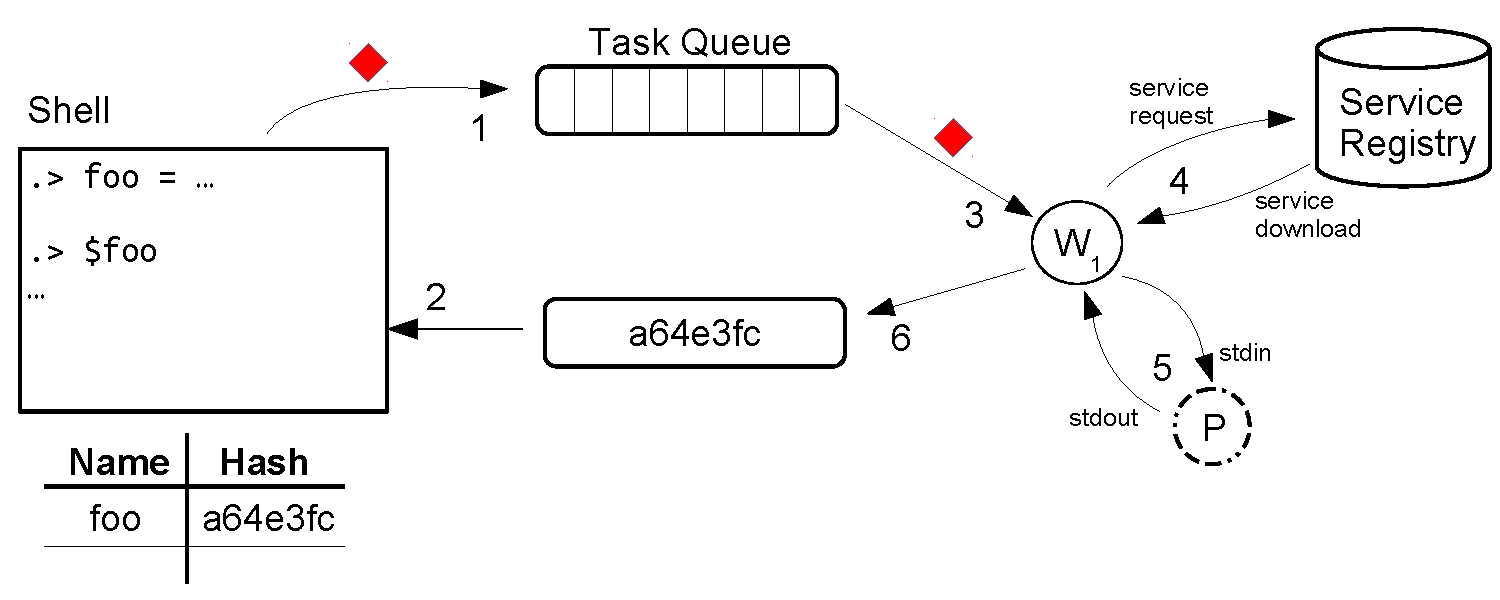
\includegraphics[scale=0.63, keepaspectratio]{system2.pdf}
  \caption{Detailed steps for processing a single task.}
  \label{system2}
\end{figure}

The command is then parsed and the task description structure
is created. If the command includes any already existing names,
the name table is used to resolve these names to their global
hashes. When the task description structure is finished, its
hash is stored in the name table behind the name \textit{foo},
as shown in the example.

Since names that are used in the command are first resolved to
their global hash names, it means that the final hash for the
task is calculated over a structure that might already contain
other hashes. Therefor the resulting hash might be a hash of hashes
and tasks issued may form a \textit{Merkle Tree} \cite{merkletree},
\cite{merkletreewiki}, in the same way that the objects stored
by \textit{Git} in its underlying file system form such a tree,
as was discussed in chapter \ref{git}.
\newline

The task is then send to the task queue, which is shown as step
1 in Fig.\ref{system2}. If the command of the user contained the
pipe operator, the shell will split the chain up into individual
commands and replace the input names of each command with the
result hash of the task description structure of its
predecessor. The individual tasks are then send to the task
queue in the order in which they are read, from left to right.
Otherwise it would be possible to construct task chaines with
more tasks then available workers, which would bring the system
to a halt.

The task queue is implemented
as a \textit{RabbitMQ} message queue \cite{rabbitmq},
\cite{rabbitmqwiki}, \cite{rabbitmqbook}. It's important to
note that the current implementation uses RabbitMQ in the
version 3.6.6-1 and that RabbitMQ is run in the fault tolerance
and distributed mode, which means that queues are replicated three
times and messages are \textit{not} written to disk but rather kept in
RAM at all times. These fault-tolerance and scalability measures
are provided by the RabbitMQ message broker by default and were
used without any modifications except for configurations and
setup.
\newline

Since the result of the command is bound to a name, a new
prompt is immediately available to the user. It is now assumed,
for the sake of the example, that the user immediately wants to
see the data of the result and therefor queries the name
\textit{foo} using the query operator \texttt{\$}. This is
shown as step 2 in Fig.\ref{system2}. This showcases another
feature that is widely adopted by most message queueing
frameworks and infrastructure: both, consumer or producer,
are able to create queues. That means that whoever requests
a queue first, will trigger its creation and any subsequent
request for queue creation are being ignored as idempotent
by the message broker. So in this case it is assumed that
the shell, as the consumer, is first to request data from the
queue with the name \textit{a64e3fc}. For step 2 it is further
assumed that no data is currently available, so no data is
printed to the user and the shell blocks in a sort of
receive loop, in the same that an actor would block, waiting
for new messages, as was introduced in chapter \ref{actorModel}.
\newline

Step 3 shows how the free worker $W_{1}$ receives the task from
the task queue. As will later be discussed in the error model
section, there is no spreading or redundant execution used in
order to deal with possible worker failure. A task must only
be received by a single worker and must also only be executed
\textit{exactly once}. This is another invariant of the system.
Guaranteeing that only exactly one worker receives a task
from the task queue is again already taken care of by RabbitMQ out
of the box. The internal queue scheduler used by RabbitMQ
uses round-robin scheduling by default. Therefor a new task
is only sent to exactly one worker. If that one fails, another
different worker will receive the task. A task is only ever
worked at by exactly one worker at a time.

The worker itself has no idea about the possible services
that are available in the system. The worker has been implemented
as a \textit{generic} worker. This means that the worker downloads
the service that is being contained in the task description from
the service registry and simply executes the received service, as
is demonstrated by step 4.

Since the generic worker is currently also written in Java,
the downloaded service could also just be Java code and therefor
executed by the worker instance natively. However, for the sake
of the example it is assumed that the downloaded service code
contains instructions to fork another Linux process. This means
that arbitrary executables can be executed by the worker, in
the same way that the foreign function interface of Cuneiform
allows to execute already existing bioinformatic tools without
any code modifications, as was introduced in chapter \ref{cuneiform}.
However, it needs to be said, that the current implementation
assumes that the binaries referenced are
already pre-installed on the worker node. However, this could be
easily avoided by also storing the needed executable in the service
registry and downloading it if necessary.
\newline

Step 5 shows how the worker has forked another Linux process.
The \textit{stdin} and \textit{stdout} (and \textit{stderr})
channels of the spawned process are redirected by the worker.
This allows the worker to receive any needed input from other
data queues in the system and forward them to the forked process
and receive any output of the forked process and forward this
output to the output queue of the worker and therefor the output
queue of the task. The forked process at no point needs to know
that it's being part of a distributed system of workers and
distributed message queues. This means already existing tools
can be re-used without any modification.
Step 6 shows how the worker forwards any piece of data
received from the forked process to the output queue, whose
name is the hash of the task description the worker received
in step 3. Whenever the worker produces an output data token,
anyone listening on this particular output queue will be able
to observe the data and so naturally the shell, as one such
listener would print the received data to screen.
\newline

Unfortunately there is a problem. Fig.\ref{system3} shows an
example including a data dependency between the task whose
result is stored behind the name \texttt{bar} and the task
whose result is stored behind the name \texttt{foo} because
the service \texttt{Cat} takes the data from \texttt{foo}
as input. Given the eager-evaluation of the shell, however,
there are multiple timings in which these
tasks might be invoked.

One would assume that the easiest one would be for the user
to take a break after she issued the \texttt{foo} command and
start the \texttt{bar} command only after the \texttt{foo}
has already finished and produced all its output data.
Then all the data would be ready even before the second task
is started, which could result in the same worker executing
both tasks. Unfortunately this is the most problematic case.

The ``best'' case in terms of implementing the data layer
using message queues only would actually be if the user
issued both commands immediately and the consuming worker,
worker $W_{2}$, was already consuming before the first data
item produced by $W_{1}$ arrived in queue \texttt{a64e3fc}.

\begin{figure}[h]
  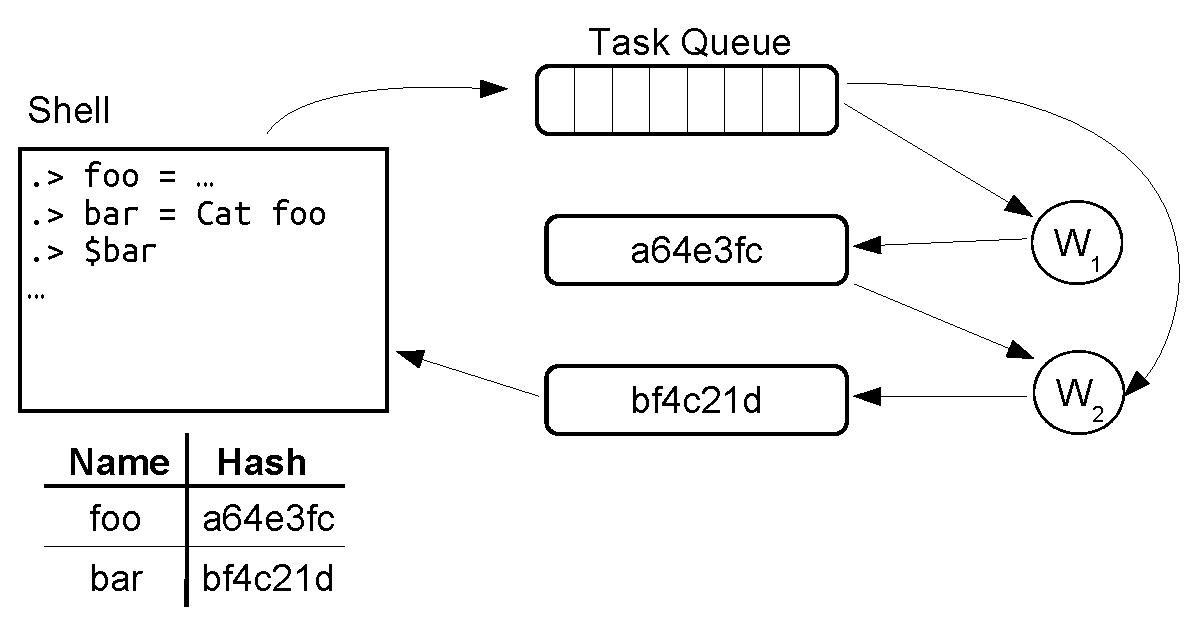
\includegraphics[scale=0.63, keepaspectratio]{system3.pdf}
  \caption{Example showing the data dependency between tasks.}
  \label{system3}
\end{figure}

This is due to the \textit{Abstract Message Queue Protocol}
(AMQP) which is implementing by almost all message queue
implementations and frameworks. The AMQP defines that,
although messages can be fanned out to multiple consumers,
a consumer only receives those messages that arrived in the
queue \textit{after} the consumer registered at the queue.

Since RabbitMQ implements the AMQP, it would've been impossible
to implement the data layer using RabbitMQ only, given the
eager-evaluation strategy of the Drift language because as was
described earlier, it must be possible for consumers to pull
data from a queue \textit{after} that data has already been
produced to that queue. In fact, consumers need to be able
to start consuming from the beginning of the queue, no matter
how much messages are already contained in that queue.

Luckily...





% consumer kommt später als producer/data
% sieht erst das was kommt, seit dem zeitpunkt des erscheinens
% brauch möglichkeit die history der queue auschecken zu können, von
% anfang an
% -> gibt AMQP nicht und damit RabbitMQ nicht her
% enter Kafka ...
